\customchapter{INTRODUCCIÓN}

\introsection{Presentación del tema de investigación}

Las heridas abiertas en la piel constituyen una de las principales causas de
consulta en los servicios de emergencia. En 2021, en Estados Unidos, se
registraron más de 722{,}000 visitas al área ambulatoria por cortes y heridas
abiertas en extremidades superiores en hombres; asimismo, Canadá reportó
aproximadamente 151{,}000 visitas por lesiones similares entre marzo de 2023 y
abril de 2024, lo que equivale a un promedio de 400 casos diarios
\cite{Informe_emergencia_2021,CIHI}. En conjunto, estas cifras evidencian una
alta demanda asistencial y, por tanto, la necesidad de optimizar los
procedimientos médicos asociados a este tipo de lesiones.

Uno de los procedimientos más empleados es la sutura, una técnica esencial para
el cierre de incisiones en tejidos blandos o heridas abiertas, tanto en
cirugías como en atención ambulatoria \cite{Instru_quirurgica}. Cuando se
ejecuta de forma adecuada, favorece la cicatrización y contribuye a prevenir
complicaciones posteriores; por ello, su correcta aplicación resulta
determinante para la seguridad y el bienestar del paciente.

No obstante, como ocurre en otros procedimientos clínicos, la sutura no está
exenta de riesgos. La complejidad de la herida, las condiciones del entorno y
la pericia del profesional influyen directamente en la aparición de
infecciones, dehiscencias o necrosis cuando no se emplean técnicas y materiales
apropiados \cite{GONZALEZ-CELY2018}. En respuesta a estas limitaciones, en los
últimos años se han propuesto diversas innovaciones orientadas a mejorar el
proceso de sutura, entre ellas el desarrollo de hilos especializados, técnicas
de cierre sin costura y el uso de fármacos que aceleran la cicatrización.

En este marco, la robótica quirúrgica y los sistemas teleoperados han cobrado
relevancia al ofrecer mayor precisión en la manipulación e incrementar el
control durante la intervención. Sistemas como Da Vinci y Zeus han contribuido
a la realización de procedimientos menos invasivos y con mayor exactitud
\cite{DaVinci,DaVinci_tumor_2024}. Además, robots especializados, como
NeuroMate (neurocirugía) y Robodoc (ortopedia), han sentado precedentes sobre
el uso de plataformas robóticas en el ámbito quirúrgico
\cite{Historia_de_los_robots_cirujanos}. De manera complementaria, estudios
recientes han explorado modificaciones en plataformas como IBIS para ejecutar
suturas semiautomáticas, con el objetivo de optimizar tiempos de manipulación y
reducir riesgos asociados.

Más allá de las mejoras en precisión, la incorporación de estas plataformas
también repercute en quien opera el sistema: se ha reportado que puede mejorar
el bienestar del cirujano al disminuir la fatiga percibida y el disconfort
físico durante la intervención. Por ejemplo, en un estudio basado en encuestas
a cirujanos ginecológicos (2012--2021), la cirugía asistida por robot mostró
menores puntajes de fatiga (escala visual analógica) y mayores puntajes de
confort frente a la laparoscopía convencional, además de una menor frecuencia
de dolor en regiones como cuello, hombros, espalda y manos
\cite{coronado_bienestar_2022}. Este tipo de hallazgos sugiere que la robótica
podría contribuir a mitigar factores asociados al desgaste ocupacional y al
burnout.

En síntesis, la evolución de las técnicas de sutura y la integración de la
robótica abren nuevas posibilidades para mejorar los resultados clínicos,
disminuir complicaciones y optimizar los procesos de atención.

\introsection{Descripción de la situación problemática}

Más allá de su magnitud a nivel global, expuesta en la sección anterior, las
heridas abiertas destacan también por su peso relativo dentro de los servicios
de emergencia. Según un estudio de 2018 realizado en cinco departamentos de
emergencia en Estados Unidos, estas lesiones ocuparon el noveno lugar entre los
motivos de consulta, con 2.7 millones de casos registrados
\cite{Emergency_reasons}. Este alto volumen de atención representa un desafío
para el sistema de salud, ya que concentra recursos y tiempo clínico en
procedimientos de resolución inmediata.

En este escenario, la sutura continúa siendo el método más utilizado para el
cierre de heridas. Si bien es un procedimiento efectivo, su ejecución repetida
en turnos de alta demanda puede generar carga física y mental en el personal
(médico y técnico) y aumentar la probabilidad de fatiga, errores y
complicaciones, especialmente cuando las condiciones del entorno (espacio
limitado y posturas subóptimas) no son ideales~\cite{Burnout_Espana,Burnout_Peru}.

\begin{figure}[H]
    \centering
    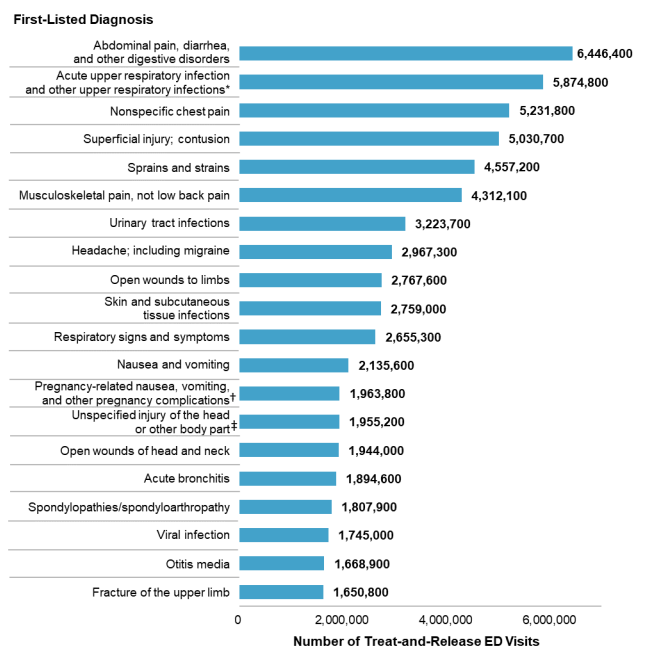
\includegraphics[width=0.75\linewidth]{images/Estadistica2018.png}
    \caption{Ranking de los 20 casos más comunes en visitas al Área de
        Emergencias en 2018\cite{Emergency_reasons}}
    \label{fig:estadistica2018}
\end{figure}

Adicionalmente, el tiempo necesario para realizar suturas varía
considerablemente según la complejidad de la herida y el área afectada
\cite{Forsch}. En escenarios de alta demanda, esta variabilidad puede prolongar
los tiempos de atención y reducir la eficiencia operativa de los servicios de
emergencia, afectando tanto la experiencia del paciente como la capacidad de
respuesta ante casos críticos.

Por ello, resulta pertinente explorar soluciones tecnológicas que estandaricen
y optimicen la ejecución del cierre de heridas, mitiguen la carga física sobre
los profesionales de la salud y reduzcan los tiempos del procedimiento. En
particular, los sistemas robóticos teleoperados con retroalimentación háptica
se perfilan como una alternativa para asistir la sutura externa, manteniendo el
control del operador y mejorando la precisión en condiciones exigentes.

\introsection{Formulación del problema}

La atención de heridas abiertas en emergencias suele requerir sutura manual, un
procedimiento que presenta limitaciones en términos de ergonomía, variabilidad
del tiempo de ejecución y dependencia de la destreza del operador. En
condiciones de alta demanda, estas limitaciones pueden traducirse en fatiga del
personal, prolongación del tiempo de atención y mayor probabilidad de eventos
adversos asociados a un cierre inadecuado
\cite{Informe_emergencia_2021,Instru_quirurgica}.

Si bien la robótica quirúrgica ha demostrado beneficios en precisión y confort
del operador en procedimientos complejos
\cite{DaVinci,coronado_bienestar_2022}, aún existe una brecha en soluciones
orientadas específicamente a la sutura externa de heridas superficiales en
entornos de emergencia, donde se requiere asistencia tecnológica sin perder el
control humano del gesto quirúrgico. En este marco, la teleoperación con
retroalimentación háptica aparece como una alternativa para mejorar la
precisión y consistencia del procedimiento, y reducir la carga física del
operador \cite{SIngle}.

Por tanto, el problema central identificado es la ausencia de un sistema
robótico teleoperado con retroalimentación háptica, específicamente orientado a
la sutura externa en heridas superficiales en entornos de emergencia, que
mantenga el control humano del gesto quirúrgico y, al mismo tiempo, mejore la
consistencia del cierre y reduzca la carga física del operador.

La solución a este problema puede transformar significativamente la atención
médica en entornos de emergencia, garantizando una mayor seguridad para los
pacientes y condiciones laborales óptimas para el personal de salud

\introsection{Objetivos de investigación}

El objetivo del presente trabajo de tesis es diseñar, integrar y controlar un
prototipo de sistema robótico teleoperado con retroalimentación háptica para la
ejecución de sutura superficial en un entorno controlado, empleando dos
interfaces hápticas y dos robots manipuladores.

\introsection{Objetivos específicos}

\begin{itemize}
    \item {Diseño y ajuste del banco de pruebas que incluye terminales de
          sujeción adaptados al módulo háptico para manipulación en entornos de sutura, y
          adaptación del efector final de los dos brazos robóticos UR5 para poder hacer
          uso de la pinza laparoscópicas genéricas.} %tangible, porcentaje avance de diseño
    \item {Comparar arquitecturas de control (optimización, SMC, impedancia)
          para el seguimiento de trayectoria del UR5 en el espacio cartesiano.}
          %tangible, avance de diseño
    \item {Establecer la arquitectura maestro-esclavo entre el Geomagic Touch
          (USB) y el UR5 (Ethernet) mediante ROS 2, con control de los grippers Robotiq
          vía Modbus RTU.}%tangible, avance de diseño
    \item {Desarrollar un sistema de teleoperación maestro/esclavo entre el
          módulo háptico y el UR5.} %tangible, avance de diseño
    \item {Integrar los módulos de teleoperación, control y hardware para
          ejecutar tareas de sutura superficial en entorno controlado.}
          %tangible, avance de diseño

\end{itemize}

\introsection{Justificación}

El departamento de urgencias médicas recibe numerosos casos de pacientes con
heridas abiertas, lo que obliga al personal médico a realizar suturas de forma
repetitiva a lo largo de su jornada. En este contexto, y en coherencia con la
formulación del problema, resulta pertinente explorar un esquema de asistencia
robótica teleoperada que mantenga al profesional en el lazo de control y
reduzca la carga física asociada al procedimiento.

Con la implementación de un módulo de teleoperación con retroalimentación
háptica, se busca mejorar la consistencia del cierre y apoyar la ejecución de
tareas repetitivas, disminuyendo la variabilidad asociada a la destreza del
operador. De este modo, se pretende mitigar molestias músculo-esqueléticas en
el personal médico y, a la vez, aportar mayor seguridad al paciente al reducir
la probabilidad de un cierre inadecuado.

La retroalimentación háptica aporta información táctil adicional a la visual,
permitiendo al operador percibir fuerzas de contacto (por ejemplo, durante el
agarre y la manipulación del instrumental) y ajustar con mayor precisión la
interacción del efector final. Con ello, se busca aproximar la sensación de
manipulación directa y facilitar una ejecución más controlada del gesto
quirúrgico.

\introsection{Alcance y limitaciones / restricciones}
% la sutura debe implicar casos de lab, las limitaciones tecnicas y biologicoas/medicas, hasta donde llegaremos con el proyecto. Limitaciones de $$, techno, alcance energético, al ser prototipo no se tendrá tanto cuidado en que plcas específicas son más econónomicas computaionlamnete.

Para el presente proyecto de tesis, se ha determinado el uso de los robots
manipuladores UR5 de Universal Robots, dado que estos se encuentran disponibles
en la universidad. En consecuencia, no se realizará una comparación formal con
otras plataformas manipuladoras para justificar su selección para tareas de
sutura.

Asimismo, se utilizará el dispositivo háptico Touch (3D Systems) como interfaz
maestra del módulo de teleoperación. Las modificaciones mecánicas y
electrónicas se orientarán a habilitar el funcionamiento del prototipo
(teleoperación y retroalimentación háptica), sin abordar en esta etapa
optimizaciones de estética, eficiencia energética o desempeño computacional.
Para el prototipado se emplearán microcontroladores y sensores disponibles en
los laboratorios del Departamento de Ingeniería Mecatrónica y Electrónica; de
no estar disponibles, se evaluará su adquisición según el presupuesto del
proyecto.

El sistema no será implementado en centros médicos. Su evaluación se realizará
en un entorno controlado mediante kits de entrenamiento usados para practicar
suturas. Se considerarán heridas superficiales y poco profundas, de tipo
limpio, de modo que el alcance se centre en validar el módulo de teleoperación
y el control del sistema, y no en abarcar la diversidad completa de escenarios
clínicos.

El proyecto será considerado exitoso si el operador logra ejecutar una sutura
superficial mediante el módulo propuesto bajo las condiciones de evaluación
definidas. Esta etapa no contempla pruebas con pacientes humanos, aunque se
espera que la experiencia obtenida sirva como base para desarrollos futuros
orientados a validaciones preclínicas y clínicas.

%